%% Why the index is not appearing?
%% Alhamdulillah, Problem fixed (21 Jan, 2021). First change compiler to MakeIndex then compile. Then compile again with XeLaTeX or PDFLaTeX.

\documentclass[11 pt]{article}


\usepackage[utf8]{inputenc}
\usepackage[table, x11names]{xcolor}
\usepackage[skins]{tcolorbox}
\usepackage[document]{ragged2e}
\usepackage[short, nodayofweek, level, 12hr]{datetime}
\usepackage[usestackEOL]{stackengine}
\usepackage[T1]{fontenc}
% \usepackage[left=2cm, right=2cm, top=2cm, bottom=3cm]{geometry}

\usepackage{multicol}

\usepackage
{
 array,
 graphicx,
 authblk,
 tikz,
 pgfplots,
 tabularx,
 mVersion,
 longtable,
 imakeidx % For creating index.
}

\usepackage[hidelinks]{hyperref}
\usetikzlibrary{patterns}
\tcbuselibrary{skins}


\setVersion{0.0}
\increaseBuild


\title{\textcolor{Firebrick4}{\textbf{Barapukuria Power Plant}}}
\author
{
	MD. MOMIN BISWAS\\
	16EEE014\\
	\href{mailto:student.bsmrstu.bdh.16eee014@gmail.com}{\textcolor{DeepSkyBlue4}{student.bsmrstu.bdh.16eee014@gmail.com}}
}
\date{21 December, 2020 \\ \currenttime \\ Version: \version}
\affil{Department of EEE, BSMRSTU}

\hypersetup
{
	colorlinks = true,
	linkcolor = blue,
	filecolor = magenta,
	urlcolor = cyan,
	pdftitle = {Barapukuria Coal Mine},
	bookmarks = true,
	hyperindex = true,
	linktocpage = false,
	breaklinks = false,
	frenchlinks = false,
}


\renewcommand\contentsname{Sections \& Sub-Sections} % Content Table
\makeindex


\begin{document}


\pagecolor{Green2}
\maketitle

\pagebreak

\pagecolor{white}

\begin{center}
	Submitted To:\index{Submitted To} \textbf{{\Large Pantha Protim Sarker}} \\
	Lecturer, Electrical and Electronic Engineering \\
	BSMRSTU, Gopalganj - 8100 \\
\end{center}

\vspace{20 mm}

Course Code: EEE369 \\
Course Title: Industrial Training

\columnseprule = 0.1 mm
\begin{multicols}{2}
There is an interface named \textit{\textcolor{blue}{Comparable}} and has a \textit{\textcolor{blue}{compare}} method at this. we can use(override) this method for our own manipulation of sorting / ordering. \textsf{Comparable} implementations provide a \textit{natural ordering} for a class, which allows objects of that class to be sorted automatically.\linebreak
If you try to sort a list, which don not implement Comparable, will throw a \textbf{\textcolor{blue}{ClassCastException}}. Similarly, \textit{Collections.sort(list)} will throw the same exception if we try to sort that list whose elements cannot be compared to one another.
\end{multicols}

\pagebreak

\tableofcontents
\pagebreak
\listoffigures

\pagebreak

\justify

\section{Depiction of Power Plant}
\index{Depiction of Power Plant}
{\huge\textcolor{red}{\hspace{5 mm}I}}n a simple manner or form a sample definition we can say that, a \textbf{Power Plant}(also known as \textbf{Power Station}) is an industrial utility station that is used to generate electrical power or an electric utility generating station. Or, in another but similar way, a \textbf{Power Plant} is an industrial location that is utilized for the generation and distribution of electric power on a massive scale. Those power plant are main source of electricity of a country's core power system. Many power stations has one or more generators, a rotating machine that converts mechanical power into three-phase electric power (these are also known as an alternator). The relative motion between a magnetic field and an electrical conductor creates an electric current.\vspace{2 mm}\\
Generally these are located in the sub-urban portion on district or several kilometers away from the public places or the load centers, because of its requisites: like as, broad land and huge water demand, along with several operating constraints like waste disposal and so on.\vspace{2 mm}\\
For this reason, a electric power generating station has to not only concern about itself with the efficient generation of the power, but also in the transmission of produced power. This is why power plants are often closely accompanied by transformer switch-yards. And these switch-yards increases the transmission voltage of the electric power, which allows it to be more efficiently transmitted over long distances.\vspace{2 mm}\\
The energy source harnessed to turn the generator shaft varies widely and are chiefly dependent on the type of fuel that are used in. The fuel choice dictates what we call the power plant, and this is how the various type of power plants are classified.
\footnote{Total Words: 276}

\pagebreak

\section{A Gallery for Power-Station}
\index{A Gallery for Power-Station}
\begin{figure}[h]
	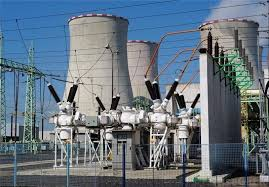
\includegraphics[width=190pt]{Gallery/One.jpg}\hspace{2 mm}
	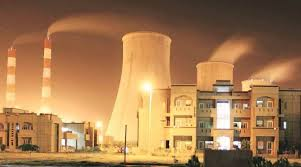
\includegraphics[width=160pt]{Gallery/Two.jpg}\vspace{2 mm}
	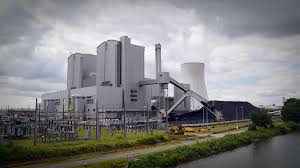
\includegraphics[width=160pt]{Gallery/Three.jpg}\hspace{1 mm}
	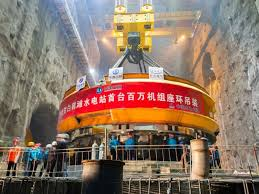
\includegraphics[width=190pt]{Gallery/Four.jpg}\vspace{3 mm}
	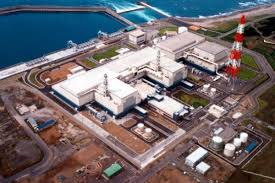
\includegraphics[width=100pt, height=50pt]{Gallery/Five.jpg}
	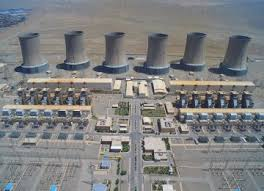
\includegraphics[width=140pt]{Gallery/Six.jpg}
	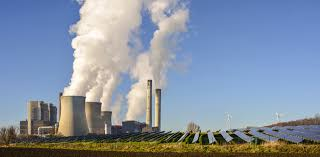
\includegraphics[width=100pt]{Gallery/Seven.jpg}
\caption{Power Plants}
\end{figure}

\pagebreak

\section{Different Types/Kinds of Power Plants}
\index{Different Types/Kinds of Power Plants}
\begin{enumerate}
	\item \textbf{Hydroelectric Power Plant:}, those are generate power by converting the force of water flow for turn to large generators.\\
And these hydroelectric Power Plants also fall into other three different categories:
		\begin{enumerate}
			\item \textbf{Impoundment:} An Impoundment facility typically used to store of a river water from a dam in a reservoir. When water is released from the reservoir, it flows through a turbine which crates motion and this turning motion activates a generator to produce electricity.\\
			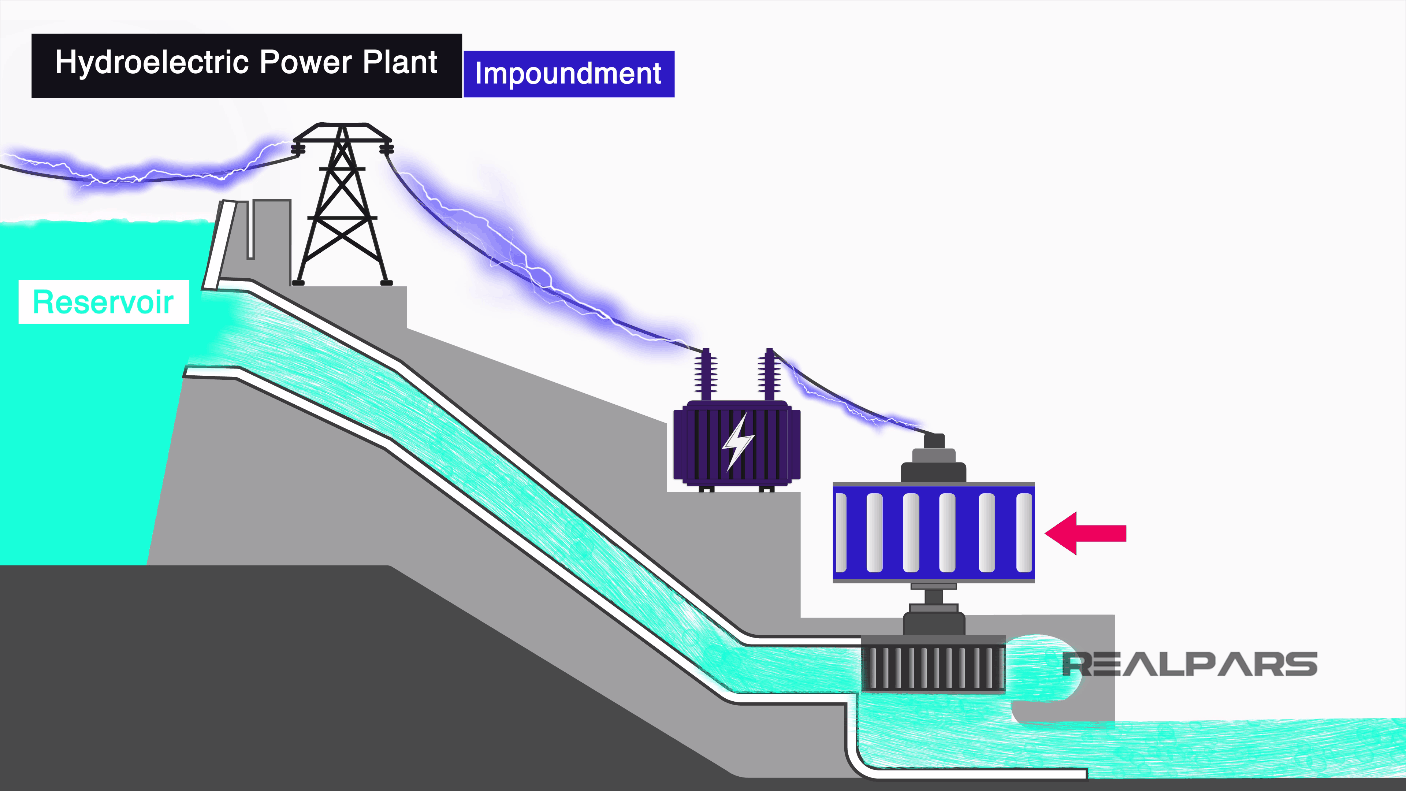
\includegraphics[width=190pt]{Gallery/Impoundment-Power-Plants.png}
			\item \textbf{Diversion:} A Diversion is fairly similar to an Impoundment facility, but may not need the use of a dam, but works by channeling a portion of a river through a canal or a penstock.\\
			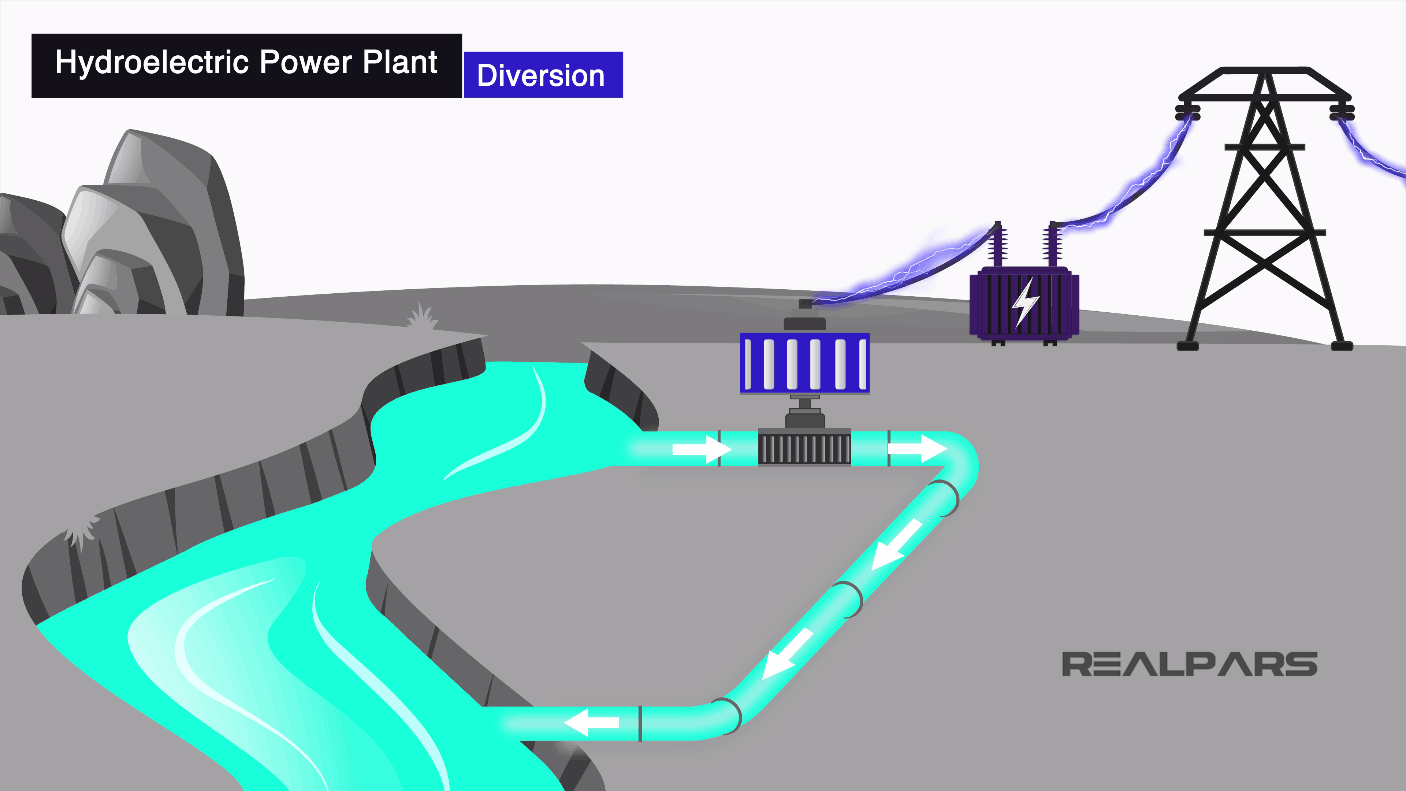
\includegraphics[width=190pt]{Gallery/Diversion-Power-Plants.png} 
			\item \textbf{Pumped Storage:} The last type of Hydroelectric Power Plant is Pumped Storage. Pumped Storage stores its energy by pumping water uphill to a reservoir at a higher elevation. When there is a demand for power, the water is released from the high elevated reservoir into a lower reservoir. This generates electricity when it flows through a turbine generating motion, and electricity.\\
		\end{enumerate}
		
		\pagebreak
		
	\item \textbf{Thermal Power Plants: }Thermal Power Plants generate electricity by converting heat into electricity, essentially by burning a fuel. Thermal power plants is one of the most important element of the energy sector and they are masterworks that enable producing electrical energy which can be thought as one of the basic needs of life after water and food. Preference of the thermal power plant's type in electricity production is a big dilemma and prior discussion subject for related parties in recent years.\\
	Thermal Power Plants fall into two different categories:
		\begin{enumerate}
			\item \textbf{Nuclear:} Nuclear power plants use reactors heat to turn water into steam. The steam is then sent through a turbine, which, as we’ve already learned, generates movement of a generator, which in turn generates electricity.\\
			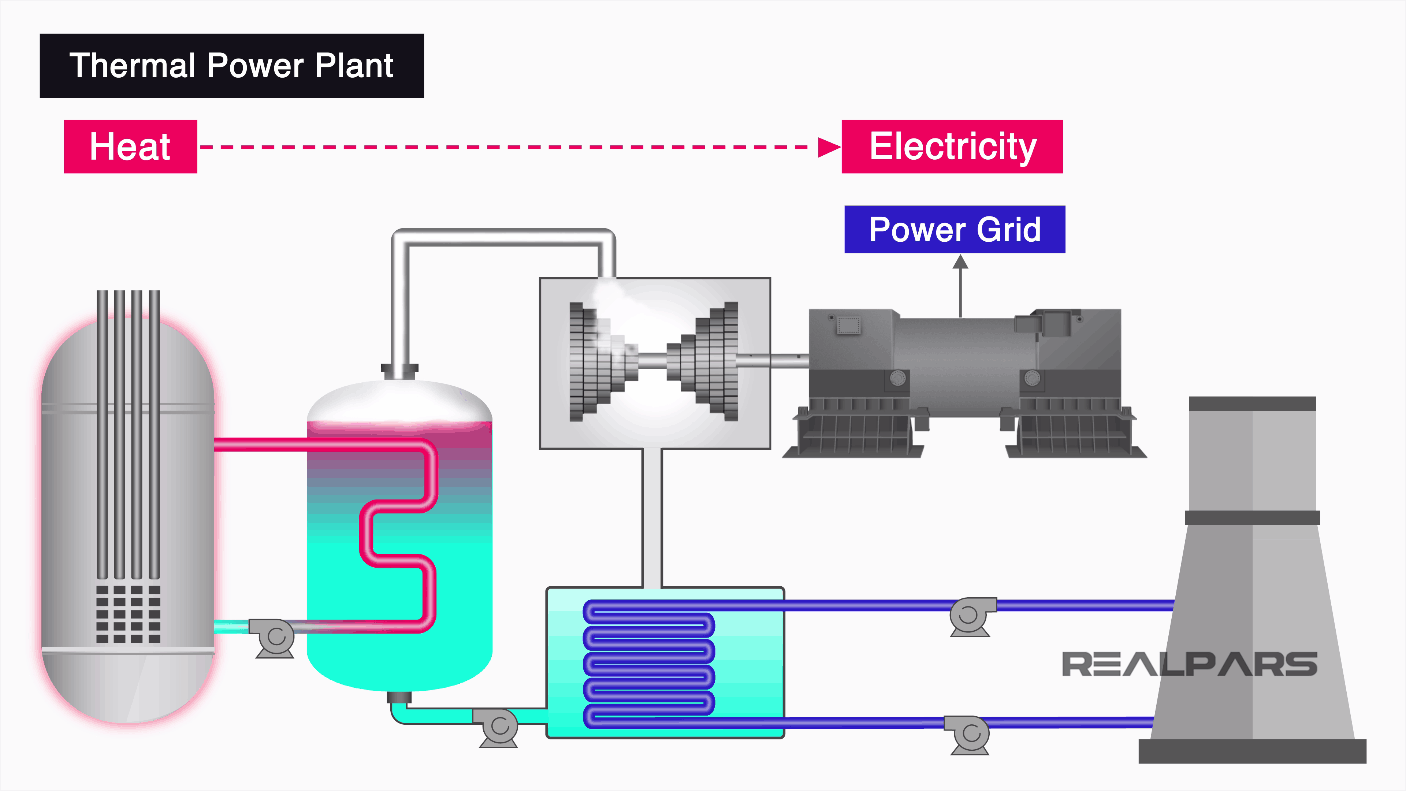
\includegraphics[width=190pt]{Gallery/Nuclear-Power-Plants.png} 
			\item \textbf{Coal:} A coal power plant works in much the same way, but instead of a nuclear reactor heating water to make steam, the heat from the burning coal powers a steam turbine.\\
			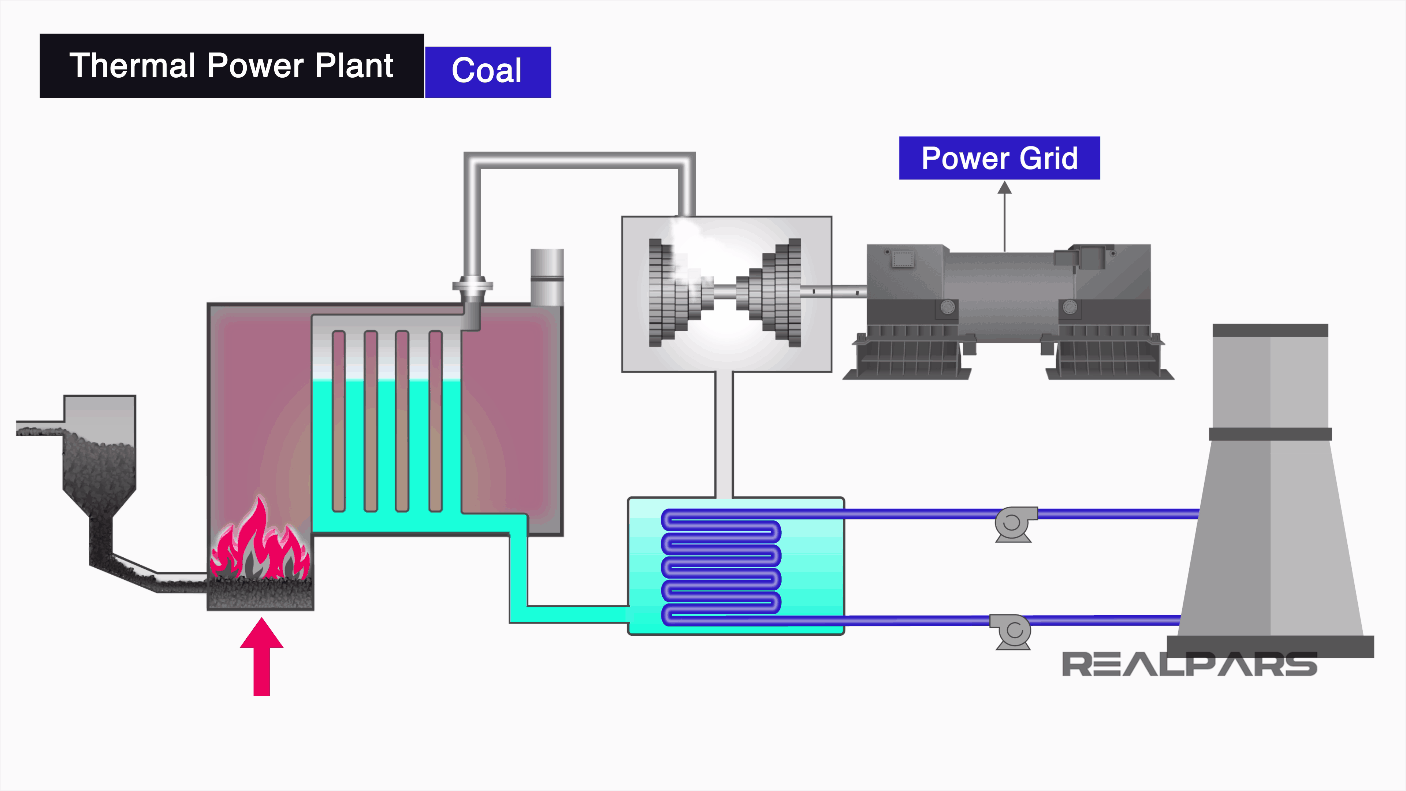
\includegraphics[width=190pt]{Gallery/Coal-Power-Plants.png} 
		\end{enumerate}
	\item \textbf{Solar Power Plants: }The next type of power plant we will look at is a solar power plant. This type of plant uses the suns energy to convert into electricity. This is achieved by using Photovoltaic, or PV panels, made up from a number of semiconductor cells that release electrons when they are warmed by the thermal energy of the sun. Solar energy is one of the cleanest ways of generating electricity. The solar panels get connected to the grid and can be used to supplement a thermal power plant resources. They can be used in domestic environments too, and with the aid of batteries, can reduce households energy consumption drastically, without burning any fossil fuels.\\
	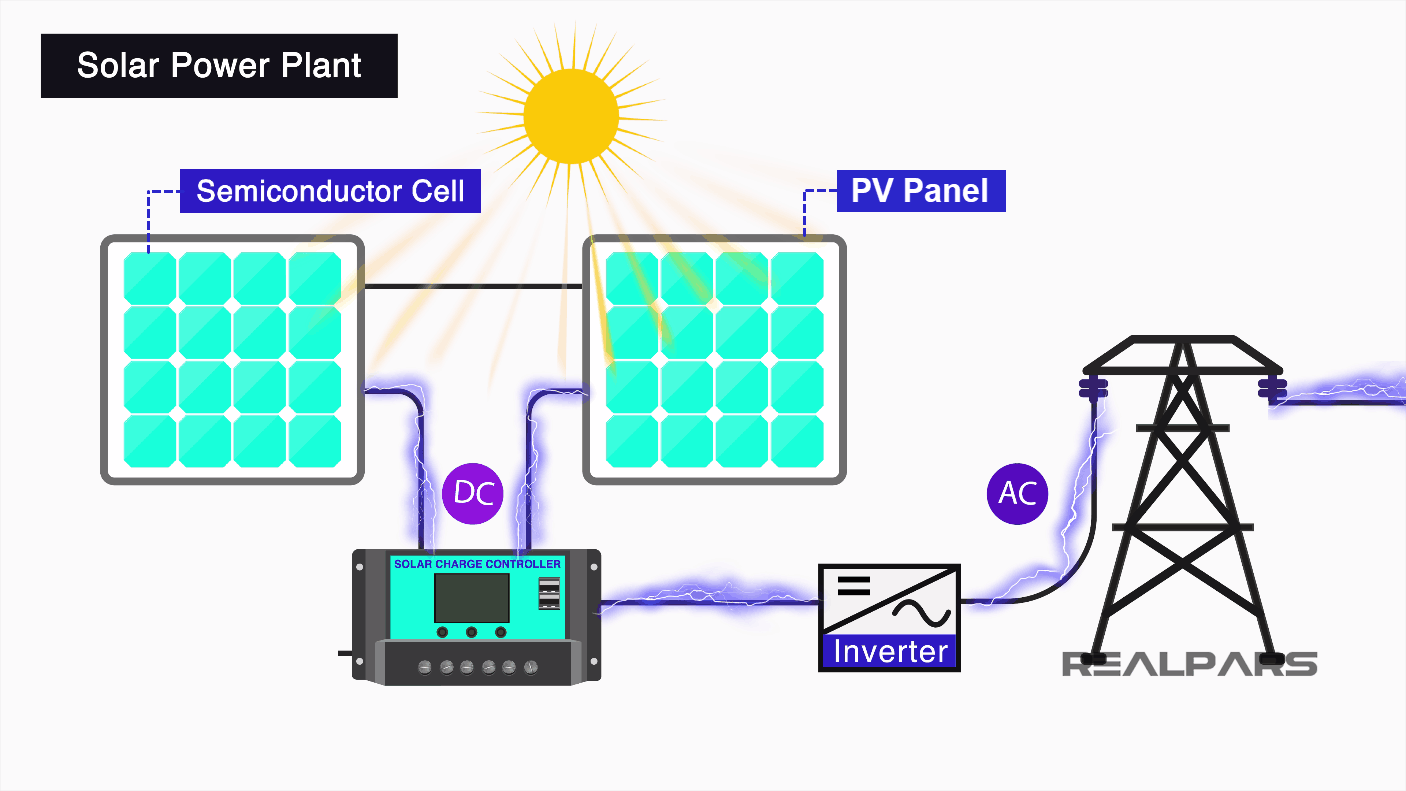
\includegraphics[width=190pt]{Gallery/Solar-Power-Plants.png} 
	\item \textbf{Wind Power Plants: }Last, but not least, we have Wind Power Plants. Wind Power Plants, or Wind Turbines, get their energy from the wind by connecting a generator to the blades. The rotational movement of the blades caused by the wind, powers a generator. Like solar power, they are a clean source of energy, but require much more hardware to work effectively, and with many more parts, are more likely to fail.\\
	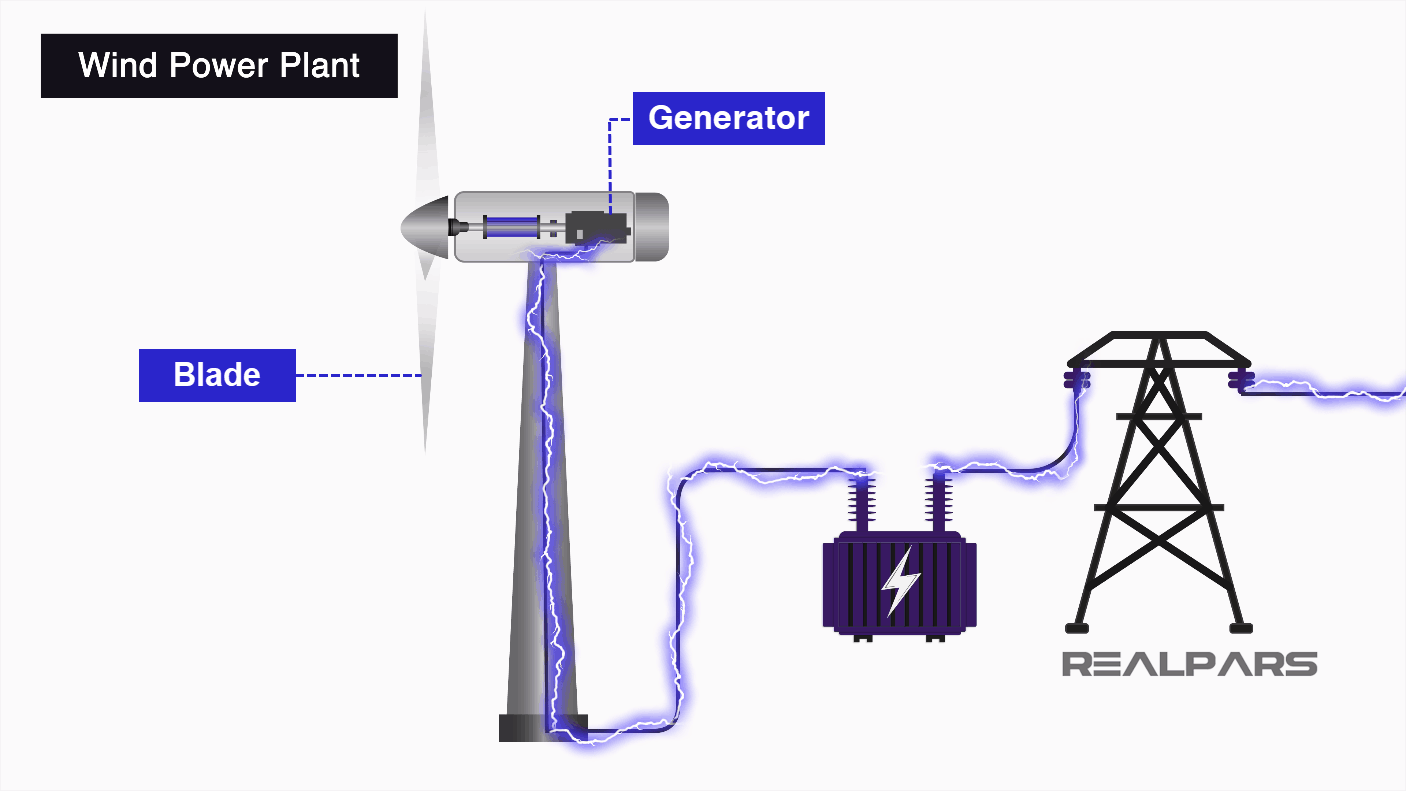
\includegraphics[width=160pt]{Gallery/Wind-Power-Plants.png}
	\hspace{2pt}
	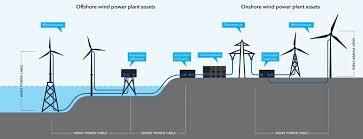
\includegraphics[width=160pt, height=108pt]{Gallery/wind power plnt.jpg}
\end{enumerate}

\pagebreak

\begin{center}
	\textit{After All Topic:} \textbf{\LARGE{\textcolor{violet}{Barapukuria Power Station}}}
\end{center}

\section{General Description and History}
\index{General Description and History}
\subsection{Starting}
\textbf{{\huge\textcolor{red}{\hspace{5 mm}B}}arapukuria Power Station} is located near Durgapur at Dinajpur in Bangladesh. It consists of two $125$ megawatt units and one $275MW$ unit. This coal-fired power station was commissioned in $2006$, and is operated by the \textit{Bangladesh Power Development Board} \textbf{(BPDB)}.\\
There are three units of the plant, operated by \textbf{BPDB}, which are jointly able to generate \large{\textit{$525MW$}} power. Two units are capable of generating \large{\textit{$250MW$}} power together and third unit can generate \large{\textit{$275MW$}} power which is synchronised with national from late December $2017$.\\
The power plan was shut down after the discovery of \textit{Barapukuria coal scam} in $22$ July, $2018$, due to acute shortage of coal. Before the shut down of the plant it had been supplying around \large{\textit{$380MW$}} power to the national grid on an average.\\
When the power plant shutdown in first time, the people of eight northern districts of Rangpur and Dinajpur regions suffered most lacking of electricity. After the consideration of their suffering, BPDB decided to restart one of its units for five days from August $20$ to lessen public suffering. On $28$ August in $2018$; the plant shut down again.

\subsection{Brief Background History}
{\huge\textcolor{red}{\hspace{5 mm}I}}{\small n 1985, Geological Survey of Bangladesh (GSB) discovered high quality bituminous Coal at a depth ranging from 118 to 509 m in \textbf{Barapukuria} under \textbf{Parbatipur Upazilla} in the district of \textbf{Dinajpur}. During 1987-1991, a UK based organization M/s Wardell Armstrong carried out the techno-economic feasibility study on this coal reserve under ODA financial support programme. Based upon the Wardell Armstrong report, Petrobangla undertook Barapukuria Coal Mine Development Project and the Project Plan (PP) was approved by ECNEC on April 21, 1993.\\
After the approval of the Project, a Construction Contract under supplier’s credit was signed on 7th February, 1994 between China National Machinery Import and Export Corporation (CMC) and Petrobangla with a view to develop an underground mine having a capacity of 1.00 Million Metric Tons of coal per annum. To ensure proper implementation of the project and smooth functioning of the mine operation Barapukuria Coal Mining Company Limited (BCMCL) was formed and registered on August 04, 1998 under the Companies Act 1994 of Bangladesh.\\
After substantial completion of the project, the mine was taken over from the Contractor (CMC) on June 30, 2005 issuing a Conditional Acceptance Certificate. A Management, Production and Maintenances Service Contract (M\&P Contract) was initialed between BCMCL and a consortium of CMC and Xuzhou Coal Mining Group Company Limited (XMC) and commercial production of coal commenced on September 10, 2005. The term of this M\&P Contract was 71 months and during this period a total production of 4.75 Mt was planned to be achieved. The contract term completed on 10.08.2011 with a total production of 3.651 Mt of coal. For continuous production of coal from the mine, a new M\&P Contract has been signed between BCMCL and CMC-XMC Consortium. Term of this contract commenced from 11.08.2012 and will remain effective for a period of 72 months with total target coal production of 5.5 Mt.}

\begin{figure}[h]
\centering
\begin{tcolorbox}[width=330pt, colframe=red, colback=green!30, arc=1.9 mm]
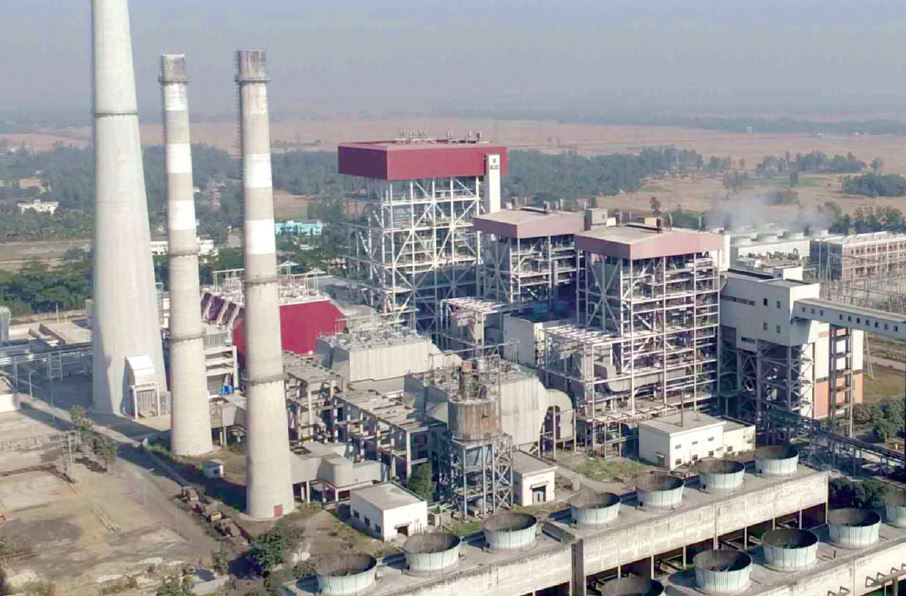
\includegraphics[width=300pt, height=180pt]{Gallery/boropurkuria thermal power station.JPG}
\end{tcolorbox}
\caption{Barapukuria Thermal Power Plant \textit{(Top-North View)}}
\end{figure}
\pagebreak

\section{Others Description in a Table}
\index{Others Description in a Table}
\begin{center}
\rowcolors{3}{green!35}{green!70}
\arrayrulecolor{white}
\columnseprule = 0.5 mm
	\begin{longtable}{|| m{14 em} || m{15 em} ||}
		\hline\hline
		\rowcolor{teal!20}
		\multicolumn{2}{c}{\textbf{\textsf{\textcolor{black}{Brief Description By \textbf{RawTable}}}}}\\
		\hline\hline
		 Gross Capacity & 525 MW(Units 1 \& 2: 125 MW, Unit 3: 275 MW)\\
		 Design Capacity & $250$ MWe\\
		 Firm Capacity & $220$ MWe\\
		 Power Plant Type & Coal\\
		 Coal Source & Boropukuria Coal Mine\\
		 Fuel Type & Coal Bituminous\\
		 Type of substation & Step-Up X Former\\
		 Supplied voltage(for 125 MW) & 13.8 KV - 230 KV\\
		 Supplied voltage(for 275 MW) & 20 KV - 230 KV\\
		 Grid Connection & 230 KV\\
		 Generation voltage & 13.8 KV - 230KV\\
		 Source of financing & Unit 3:US \$$224$ million\\
		 Type of plant & Sub-critical Thermal\\
		\hline\hline
	\end{longtable}
\end{center}

\section{Cycle Description}
\index{Cycle Description}
{\huge\textcolor{red}{\hspace{5 mm}B}}arapukuria, Parbotipur in January, 2006. The plant is operated under Bangladesh Power Development Board (BPDB), which consists of 2 units (2 x 125 MW). This plant is operating on sub-critical steam conditions. Coal fired thermal power plant generally operates on Rankine cycle. The schematic arrangement of equipments of this power plant is shown in Fig. 
The major components of the plant are high, intermediate and differential low-pressure turbines (HPT, IPT and DFLP), boiler (B), pumps (P), deaerator (D), generator (G), condenser (C), low and high-pressure feed water heaters etc. The thermodynamic models of this power plant are based on fundamental mass, energy and exergy balances. Using the mass, energy and exergy balance equations for each component of the power plant, it is possible to compute energy and exergy flows at each node of the plants, energy and exergy efficiencies and irreversibilities of the component and so on.  Yet, the mature CO2 capture technologies result in net efficiency penalties of at least 7\% points. Emerging technologies, such as calcium looping combustion, can reduce the net efficiency penalty to 2.4\% points. Further reductions can be achieved by replacing the conventional steam cycle with advanced power cycles. This study aimed to assess the techno-economic feasibility of the coal-fired power plant based on calcium looping combustion with different advanced Brayton cycles. These included single power cycles, such as recompression supercritical CO2, simple supercritical CO2 cycle, and xenon cycle, as well as combined power cycles based on helium, nitrogen and recompression supercritical CO2 cycles. The net efficiency and break-even electricity price, which was estimated using the net present value method, were used as the key techno-economic performance indicators. A parametric study was also conducted to assess the impact of the key thermodynamic parameters. trofits, the coal-fired power plant based on CaLC was shown to be characterised with 37\% higher break-even cost of electricity than that of the coal-fired power plant without CCS (59.63 €/MWel,neth,neth) . Such an increase was shown to be lower than that for an amine scrubbing retrofit (62\%) and CaL retrofit (44\%).Further improvement in the techno-economic feasibility of the coal-fired power plant based on CaLC can be achieved through revision of the sCO2 cycle structure and operating conditions, as well as consideration of other advanced power cycles, such as closed Brayton cycles (CBC) using different working media. These power cycles are currently at a lower maturity level than the conventional steam cycle. Although application of these advanced power cycles has been evaluated for nuclear power plants and solar power plants, their application to coal-fired power plants has not been considered, with the exception of the sCO2 cycle.Therefore, this study proposes to integrate the advanced power cycles with CaLC for high-efficiency power generation with low CO2 emissions and affordable cost of electricity. To assess the techno-economic feasibility of the proposed designs of the coal-fired power plant based on CaLC, process models for each advanced power cycle were developed in Aspen Plus® and validated with the data available in the literature, before integration with CaLC. The techno-economic performance was assessed considering the net efficiency and the break-even price of electricity (BEPel).Steam flows to HP Turbine (point 1) with high energy and high exergy, after producing work on expansion in HP turbine, cold reheat steam (point 12) with low energy and exergy flows back to boiler for reheating, hot reheat steam (point 3) with high energy and exergy flows to IP turbine and then LP turbine, where further expansion takes place and work is produced.

\section{Basic Engineering}
\index{Basic Engineering}
{\huge\textcolor{red}{\hspace{5 mm}I}}n a Coal-fired thermal plants produce electricity by burning coal as fuel which produces tremendous heat. After that, the heat produces steam. The steam induces a great pressure and flows into turbine  making it rotate with the generator cooled with the turbine. Thus the rotation of generator generates electricity. The steam is then cooled and condensed back into water and goes back to the boiler to start over the process again.

\pagebreak

\section{Connection To Grid}
\index{Connection To Grid}
\rowcolors{2}{blue!9}{gray!20}
\arrayrulecolor{white}
	\begin{longtable}{|| m{10 em} | m{10 em} ||}
		\hline\hline
		\rowcolor{teal!20}
			\hline
			\rowcolor{green!70}
			\textbf{\textit{Name}} & \textbf{\textit{Rating}} \\
			\hline\hline
			Generation Voltage & 125MW = 13.8 KV \\
			\hline
			Generation Voltage & 175MW = 20 KV \\
			\hline
			\multicolumn{2}{c}{Total Grid Voltage - 230 KV} \\
			\hline\hline
	\end{longtable}

\begin{figure}[h!]
\centering
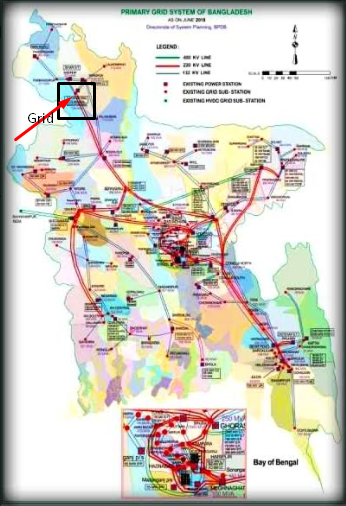
\includegraphics[width=\textwidth-110pt, height=300pt]{Gallery/Grid.png}
\caption{Connection Grid}
\end{figure}

\pagebreak

\section{Operation}
\index{Operation}
\subsection{Operation Of A Thermal Power Plant}
{\huge\textcolor{red}{\hspace{5 mm}A}}s far as we know, \textbf{Barapukuria Power Plant} is a thermal power plant. Here I'm just discussing about the operation of thermal power plant.\\
Operation of \textbf{Thermal Power Plant} depends on \textbf{Rankin Cycle}. In a thermal power plant, coal storage provides coal and burnt in the boiler section. Main task of it, converting water into steam. This steam is expanded in the turbine which produces mechanical power driving the alternator coupled to the turbine. The steam is expanded again the turbine and usually condensed in the condenser to be fed into the boiler. But in real practice, the conversion of heat from coal combustion into electrical energy needs some modern arrangements and improvements, in which it will run in proper working efficiency. Here are some basic circuit arrangements of the modern thermal power plant operation.\\

\subsection{Operation Of Barapukuria Power Plant}
{\huge\textcolor{red}{\hspace{5 mm}B}}arapukuria Coal Based Thermal Power Plant is the steam turbine power plant. Electrical energy generation using steam turbine involves three energy conversions.First, the extraction of heat energy from fuel, in this case it is coal. Then use that thermal energy of steam to convert the kinetic energy to rotate the turbine. Finally, convert the mechanical energy of the turbine into electrical energy using a generator. In Barapukuria power station, the steam is produced by burning coal in a combustion chamber. The chemical process of burning fuel releases heat. That heat is being used to create steam from the boiler. The steam has high kinetic energy.The turbine is rotated by directing high temperature steam. The turbine is coupled with the rotor of a generator which converts mechanical energy into electrical energy. This is the basic principle of a steam turbine power plant.

\subsubsection{Boiler}
{\huge\textcolor{red}{\hspace{5 mm}S}}team boilers are a necessary part of thermal power plants. A steam boiler is a dense vessel where water is heated until it converts to steam at the required pressure. Water is stored inside the boiler The stored fuel is burned in a furnace and hot gas is produced. The hot gases come in contact with the hydraulic vessel where the heated gas is transferred to the heated water and steam. This high pressure steam is then piped to the turbine of the power plant.\\
Weather tubes carry water or flue gas, depending on that, boilers is of two types:
\newenvironment{myitemize}
{\begin{itemize}}{\end{itemize}}
\tcolorboxenvironment{myitemize}{blanker, before skip=6pt, after skip=6pt, borderline west={3mm}{0pt}{yellow}}
\begin{myitemize}
	\item Fire tube boiler
	\item Water tube boiler
\end{myitemize}
\vspace{4 mm}
In Barapukuria, the boiler is of
\begin{myitemize}
	\item water tube type
	\item internal combustion type
	\item high pressure type
	\item natural circulation type
	\item single drum type
\end{myitemize}
\vspace{4 mm}

\textbf{Water Tube Boiler: } In water tube boilers, water is heated inside the tube and hot gases surround them. This is the opposite of a fire tube boiler. In water tube boilers, the vapor pressure is higher than in fire tube boilers. 
\textbf{Internal combustion boiler: } Combustion of fuel and hot air occurs inside the boiler. This type of boiler produces hot gas from the inside of the boiler.\\
\textbf{High pressure boiler: }A high pressure boiler has a high vapor pressure and a temperature of more than 250 degrees Celsius.\\
\textbf{Natural circulation: }The natural circulation of water by conventional currents or gravity circulation.\\
\textbf{Single drum boiler: }Single drums are used to store demi water. Multiple drums are positioned.\\

\pagebreak

\begin{center}
\rowcolors{2}{red!20}{red!60}
\arrayrulecolor{white}
	\begin{longtable}{|| m{18 em} | m{7 em} ||}
		\rowcolor{teal!20}
		\multicolumn{2}{c}{\textbf{\textsf{\textcolor{black}{\footnotesize{Type Single Furnace Type(Model SG-400/14.42-M772)}}}}}\\
		\hline
		\rowcolor{green!40}
			\textbf{Name} & \textbf{Rating}\\
			\hline\hline
			Maximum Continuous Rating &  400t/h\\
			Main Steam Outlet Pressure & 14.42 Mpa\\
			Main Steam Outlet Temperature & 538oC\\
			Reheated Steam Flow & 325t/h\\
			Reheated Steam Pressure (In/Out) & 2.31/2.21 Mpa\\
			Reheated Steam Temperature (In/Out) & 290oC/538oC\\
			Fuel Bituminous & Coal\\
			Combustion & 4 corner firing\\
			Feed Water Temperature & 248oC\\
			Rated Power & 125 MW\\
		\hline\hline
	\end{longtable}
\end{center}

\subsubsection{Manufacturer Shanghai Boiler Works Limited}
{\huge\textcolor{red}{\hspace{5 mm}T}}his boiler has 6 furnace beds. Each furnace bed has a 4 corner firing system. The furnace bed is supplied with a mixture of hot air and coal powder. The combustion of the mixture then produces hot gas. The hot gas goes around the water tubes and the heat is transferred from the heat to the water.Feed water is preheated at 248oC. The temperature of the vapor produced in the tubes is 538oC. These are made of high-temperature steam turbine pipes. The temperature of the output stream is about 290oC which goes through the economy and is reheated for reuse. This increases the efficiency of the boiler.

\subsubsection{Steam Turbine}
{\huge\textcolor{red}{\hspace{5 mm}A}} steam turbine is a mechanical device that extracts thermal
energy from pressurized steam and converts it into mechanical
work. The main parts of stream turbines are blades and rotors.
A set of blades is known as a stage. They also have steam inlets
and outlets. Two separate processes known as governors are
used to ensure the safe operation of the turbine.\\

\pagebreak

There are two basic types of turbines:
\begin{enumerate}
	\item [\textcolor{violet}{Impulse turbine:}]In emuls turbines, high-pressure steam is thrown through a narrow nozzle to spin on the turbine blades. The blade of an impulse turbine is usually bucket shaped. In an impulse turbine, steam is forced to hit the turbine at high speeds. High-speed steam from the nozzle kicks in the blades and pushes them around with constant persuasion.
	\item [\textcolor{violet}{Reaction Turbine:}]In a reaction turbine, a second set of stable blades is attached to the interior of the turbine case. As the steam hits the rotor blades, it creates a reactive force in the blades that rotates the rotating turbine rotor. The rotor basically becomes a set of rotating nozzles. The turbine used in Barapukuria is a reaction concentrated and super high pressure turbine. It has a re-heater with HP and IP cylinders. It has double casing with single trench. The rated capacity of the turbine is 125 MW. The rotation of the turbine is clockwise from the turbine to the generator.The speed of the turbine is 3000 RPM.
\end{enumerate}

\subsubsection{Alternator at Barapukuria power plant}
{\huge\textcolor{red}{\hspace{5 mm}A}}n alternator is an electric generator or device that converts to the mechanical energy into an electrical energy. For simplicity most alternator stores use the magnetic field as a rotor and armeture as a stator. Alternators at power stations are powered by turbines or engines.The alternator used in Barapukuria power plant is Type QFS-125-2. It is a 2 pole generator. Rated capacity in KVA is 156250. Active power of the generator is 125 MW. Stator voltage is 13.8 KV. Stator current is 6537 A. The rotor current at no load condition is 627 A and at load is 1750 A. Rotor voltage at no load condition is 88 V and at load is 275 V. The speed of the alternator is 3000 RPM which generates at 50 Hz current. The manufacturer is Shanghai Turbine Generator Company Limited (STGCL).
\subsubsection{Transformer}
{\huge\textcolor{red}{\hspace{5 mm}A}}n electric power transformer is a device that converts electrical energy from one circuit to another. It converts electrical voltages at different levels without changing the frequency. The transformer used in Barapukuria power station is a step up transformer.The rating of the transformer used in Barapukuria is 13.8 KV/230 KV. The manufacturer of the transformer is Baoding Tianwei Baodian Electric Company Limited (BTBECL). The cooling system of the transformer is oil filled cooling system. MVA rating is 156.25 MVA. This is a three phases transformer with ONAF system. ONAF is oil forced air forced cooling of transformer. The generated voltage of Barapukuria power plant is 13.8 KV and the supply voltage of the power station to the grid is 230 KV.
\subsubsection{Cooling Systems}
{\huge\textcolor{red}{\hspace{5 mm}T}}he cooling system in Barapukuria power station is a type of water cooling. There are cooling towers and fourteen deep tube wells for this cooling system. The amount of cold water used per day is 800-1000 metric tons. Cooling tower is a heat rejection device that removes heat from the equipment into the atmosphere through water vapor. Cooling towers remove heat by circulating water through a water jacket. For this reason there is a capacity full of water, to purify this water lots of chemical is used in it. This water is continuously piped to the de-mineralized tank. Water circulates inside the system in water jackets around boilers, turbines, etc. To keep the temperature at a reasonable level, the jacket is left and the hot water is sent to the heat exchanger. Raw water flows through the heat exchanger, where it absorbs the water heat of the jacket. It then cools in the cooling tower and spreads again.

\section{Power Generation Data form Recent Two Years}
\index{Power Generation Data form Recent Two Years}
\subsection{2018 - 2019}
\rowcolors{1}{white}{white}
\arrayrulecolor{black}
	\begin{longtable}{| m{0.8 em} | m{4 em} | m{1.5 em} | m{4.5 em} | m{4 em} | m{2.2 em} | m{3.1 em} | m{4 em} |}
		\hline\hline
		\rowcolor{teal!20}
		\multicolumn{8}{c}{\textbf{\textsf{\textcolor{black}{Power Generation}}}}\\
		\hline\hline
		\rowcolor{blue!50}
			\footnotesize{SI.} & \footnotesize{Name Of Power Plant} & \footnotesize{Type Of Fuel} & \footnotesize{Installed Capacity(As of June)(MW)} & \tiny{Net Energy Generation(GWh)} & \tiny{Annual Plant Factor(\%)} & \tiny{Efficiency(\%)} & \tiny{Overall Thermal Efficiency(\%)(Net)}\\
		\hline\hline
		1. & \tiny{(a)Barapukuria TPP Unit-1,2} & {\footnotesize Coal} & 250 & 103.4305 & 8.46 & 19.36 & 38.4\\
		\hline
		2. & \tiny{(b)Barapukuria 275MW TPP Unit-3} & {\footnotesize Coal} & 274 & 1126.0726 & 52.32 & 32.39 & 38.4\\
		\hline\hline
	\end{longtable}
\pagebreak
\subsection{2019 - 2020}

\rowcolors{2}{white}{white}
\arrayrulecolor{black}
	\begin{longtable}{| m{0.8 em} | m{4 em} | m{1.5 em} | m{4.5 em} | m{4 em} | m{2.2 em} | m{3.1 em} | m{4 em} |}
		\hline\hline
		\rowcolor{teal!20}
		\multicolumn{8}{c}{\textbf{\textsf{\textcolor{black}{Power Generation}}}}\\
		\hline\hline
		\rowcolor{blue!50}
			\footnotesize{SI.} & \footnotesize{Name Of Power Plant} & \footnotesize{Type Of Fuel} & \footnotesize{Installed Capacity(As of June)(MW)} & \tiny{Net Energy Generation(GWh)} & \tiny{Annual Plant Factor(\%)} & {\tiny Efficiency(\%)} & \tiny{Overall Thermal Efficiency(\%)(Net)}\\
		\hline\hline
		1. & \tiny{(a)Barapukuria TPP Unit-1,2} & {\footnotesize Coal} & 250 & 307.46 & 23.8 & 25.52 & 37.8\\
		\hline
		2. & \tiny{(b)Barapukuria 275MW TPP Unit-3} & {\footnotesize Coal} & 274 & 1759.57 & 80.60 & 34.23 & 37.8\\
		\hline\hline
	\end{longtable}
	
\pagebreak

\subsection{Generation Cost}
\subsubsection{2018 - 2019}
\rowcolors{2}{green!20}{gray!40}
\arrayrulecolor{white}
	\begin{longtable}{|| m{5.1 em} || m{8 em} || m{7.5 em} || m{5.5 em} ||}
		\hline\hline
		\rowcolor{teal!20}
		\multicolumn{4}{c}{\textbf{\textsf{\textcolor{black}{Generating Plant Under Power Station}}}}\\
		\rowcolor{blue!60}
		\hline\hline
		    \hline
			 & {\footnotesize Barapukuria Power Station Unit-1, 2} & {\footnotesize Barapukuria Power Station Unit-3} & {\footnotesize Total Coal}\\
			\hline
			\footnotesize{Capacity} & 220 & 274 & 494\\
			\footnotesize{Plant Factor} & 5\% & 47\% & 28\%\\
			\footnotesize{Net Generation(kWh)} & 103,430,490 & 1,126,072,607 & {\small 1,229,503,097}\\
			\footnotesize{Fuel Cost} & 540,564,685 & 5,885,257,664 & {\small 6,425,822,348}\\
			\footnotesize{Fuel Cost(Tk/kWh)} & 5.23 & 5.23 & 5.23\\
			\footnotesize{Variable(O\& M TK.)} & 23,807,646 & 259,199,569 & {\small 283,007,215}\\
			\footnotesize{Variable(O\& M TK./kWh)} & 0.23 & 0.23 & 0.23\\
			\footnotesize{Total Fixed Cost(TK.)} & 888,309,643 & 2,542,688,177 & {\small 3,430,997,820}\\
			\tiny{Fixed Cost(TK./kWh)} & 8.59 & 2.26 & 2.79\\
			\footnotesize{Total Generation Cost(TK.)} & 1,542,681,974 & 8,687,145,409 & {\small 10,139,827,384}\\
			\tiny{Generation Cost(TK./kWh)} & 1.05 & 7.71 & 8.25\\
		\hline\hline
	\end{longtable}
\pagebreak
\subsubsection{2019 - 2020}
\rowcolors{2}{green!20}{gray!40}
\arrayrulecolor{white}
	\begin{longtable}{|| m{5.1 em} || m{8 em} || m{7.5 em} || m{5.5 em} ||}
		\hline\hline
		\rowcolor{teal!20}
		\multicolumn{4}{c}{\textbf{\textsf{\textcolor{black}{Generating Plant Under Power Station}}}}\\
		\rowcolor{blue!60}
		\hline\hline
		    \hline
			 & {\footnotesize Barapukuria Power Station Unit-1, 2} & {\footnotesize Barapukuria Power Station Unit-3} & {\footnotesize Total Coal}\\
			\hline
			\footnotesize{Capacity} & 220 & 274 & 494\\
			\footnotesize{Plant Factor} & 16\% & 73\% & 48\%\\
			\footnotesize{Net Generation(kWh)} & 307,464,596 & 1,759,569,881 & {\small 2,067,034,477}\\
			\footnotesize{Fuel Cost} & 1,533,006,616 & 8,773,147,554 & {\small 10,306,154,169}\\
			\footnotesize{Fuel Cost(Tk/kWh)} & 4.99 & 4.99 & 4.99\\
			\footnotesize{Variable(O\& M TK.)} & 31,064,397 & 177,776,490 & {\small 208,840,887}\\
			\footnotesize{Variable(O\& M TK./kWh)} & 0.10 & 0.10 & 0.10\\
			\footnotesize{Total Fixed Cost(TK.)} & 1,244,226,681 & 2,675,856,257 & {\small 3,920,082,939}\\
			\tiny{Fixed Cost(TK./kWh)} & 4.05 & 1.52 & 1.90\\
			\footnotesize{Total Generation Cost(TK.)} & 2,808,297,694 & 11,626,780,301 & {\small 14,435,077,994}\\
			\tiny{Generation Cost(TK./kWh)} & 9.13 & 6.61 & 6.98\\
		\hline\hline
	\end{longtable}
\pagebreak

\section{Sub-Station}
\index{Sub-Station}
\hspace{5 mm} \justify{{\huge\textcolor{red}{A}} substation is used to transfer power from the generating plant to the end consumer. It is made of equipment such as power cable, generator, and transformer, which assist in electricity transmission. A substation’s primary functions are the distribution, transmission, and generation of power. Barapukuria has to sub-station. They have use step-up x former. For unit - 1 and 2, using 125 MW and 13.82 to 230 kV. For Unit - 3, 275 MW using 20 to 230 kV.}\vspace{4 mm}\\

\begin{figure}[h!]
\centering
\includegraphics[width=360pt,height=220pt]{../../../Downloads/CYMERA_20201221_210039.jpg}
\caption{Flow Diagram Of Sub-Station}
\end{figure}

\section{Financial Feasibility}
\index{Financial Feasibility}
\subsection{Introduction}
{\huge\textcolor{red}{\hspace{5 mm}W}}e all know that \textbf{Barapukuria Power Plant} is a \textbf{Thermal Power Plant}. And a Thermal Power Plant installed for produce electrical power/energy which is a secondary energy-source by using the primary energy-sources. Followed by the \textit{International Energy Outlook Report}, marketable energy consumption in the World, taking 2007 as the root/base year, is expected to grow 49\% until 2035 (IEO, 2010). Look at the figure for obtain concept behind distribution of estimated energy consumption by primary source (According to the report).\\
\begin{figure}[h]
\caption{Estimated Energy: Distribution Graph.}
\centering
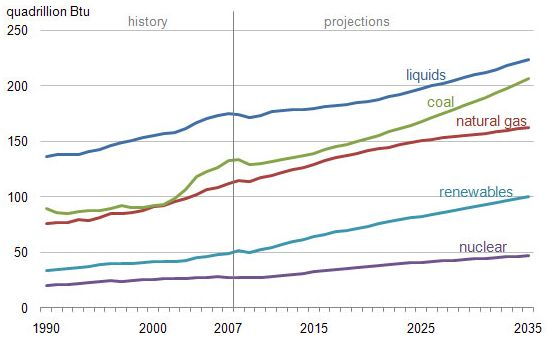
\includegraphics[width=300pt]{Gallery/report figure.jpg}
\end{figure}

Thermal power plants is one of the most important element of the energy section and they are the masterworks that enables producing electrical energy which can be thought as one of the basic needs of life after water and food precisely. Preference of the thermal power plant's type in electricity production is a big dilemma and prior discussion subject for related parties in recent years. For instance, environmentalists act against fossil-fuelled thermal power plants or nuclear power plants and they try to warn decision-makers about environmental pollution, global warming, carbon emissions etc. There is no doubt that eliminating the existence of such kind of industrial elements, playing a major role in environmental issues seems true, but only with a view of environmentalism because when many other factors were considered, thoughts of environmentalists cannot be accepted in short- or medium-term. The thoughts, agreed and supported by everyone, can be ignored suddenly and quickly because the needs, called energy, especially in economic frame, have a vital importance.

\tcbset{frogbox/.style={enhanced, colback=green!10, colframe=green!65!black,
enlarge top by=5.5mm,
overlay={\foreach \x in {2cm, 3.5cm} {
\begin{scope}[shift={([xshift=\x]frame.north west)}]
\path[draw=green!65!black,fill=green!10,line width=1mm] (0,0) arc (0:180:5mm);
\path[fill=black] (-0.2,0) arc (0:180:1mm);
\end{scope}}}}}
\begin{center}
\begin{tcolorbox}[frogbox, arc=3 mm, width= 356 pt]
	Financially: A bird in the hand is better than two in the bush.
\end{tcolorbox}
\end{center}

\subsection{Finance Behind Barapukuria Coal Mine}
\hspace{5 mm} \textbf{First Portion:} For any investment decision, it is necessary to evaluate comparative economics of the feasible technical alternatives. In the present case also, it is necessary to carry out cash flow analyses for at least next 10 years (with 1st year as 2011-12) considering a rated production of 1.0 Mtpa for the existing longwall multi-slice system and the proposed LTCC\footnote{LTCC - Longwall Top Coal Caving} system to compare the economics of these two systems.\\
For this purpose, the operating and capital costs of the existing system need to be updated and a revised cost estimate (RCE)\footnote{RCE - Revised Cost Estimate} of the existing mine should be prepared. The economics of the two systems may then be compared in terms of their Financial IRRs\footnote{IRR - Internal Rate of Return} and Economic IRRs or in terms of their NPVs\footnote{NPV - Net Present Value}.\\
Further, it is desirable to carry out sensitivity analyses of the FIRRs or NPVs of the two systems to ascertain the risks involved in each system. These financial analyses must, therefore, be carried out for both the systems before taking a final decision regarding selection of a system.\\
Considering the M\&P contract for the Barapukuria mine to be valid for a period of 5 years, these analyses may also be mapped for such a smaller period to assess the risk of disengagement of BCMCL\footnote{BCMCL - Barapukuria Coal Mining Company Limited} with the present contractor after the completion of the contractual period.\\
\textbf{Second Portion:} Investment is the base point of mining. For this reason, we need a big amount of money to get started and then we found an extended hand from China\textit{(The People's Republic of China)}. January, in the year of 2014, Chinese private bank \textit{Industrial and Commercial Bank of China} \textbf{(ICBC)} offered our country \textit{(Bangladesh)} a hard loan of \$224 million to increase the capacity of the 250MW Barapukuria coal-fired thermal power station by 275 MW. The remainder of the estimated cost of the \$330.52 million project was to be funded by the Govt. of Bangladesh. The loan comes with an interest rate of 3.98\%, a management fee of 1.5\%, an insurance premium of 6.62\% and commitment fee of 1 percent. 13 years is set as Repayment period. On 16 February - 2015, \textbf{ICBC} extended the loan to be valid beyond June 30, 2016. As of August 2, 2016, 40\% of the power plant project is complete. Harbin Electric International \textbf{(HEI)} and \textbf{CCC} contracting firm are implementing the project. And expected completion date was at June in the year of 2018.

\section{Importance}
\index{Importance}
\hspace{5 mm} {\huge\textcolor{red}{A}} country can move forward if it has a good source of Power Generation with the Transmission and Distribution system. By the amount of power generation, we can determine the country’s overall development. We will find lots of countries those who ensure a well-established power system and they are leading the world. It also can depend on many sources from where a country will generate electric power.\\
Our energy needs (electricity needs) can be met from various of sources, like so - hydel, thermal (includes fossil fuel and nuclear fuel plants), wind power, solar (PV) and so on\dots. Out of the above, wind power and solar are not reliable for continuous production of electricity - wind can die down, solar won’t work in night or when the cloud cover is too thick. Hydel plants are seasonal - they depend on rivers, dams, rains etc. Thermal power plants are the most reliable - they can work round the clock, round the year (except for occasional downtime for maintenance). It is not therefore surprising that many countries use thermal power as the base to meet the energy demand and use the other modes of energy production to supplement the thermal units. For example, some of the hydel units may be operated in the night when solar units are not available and similarly when wind power units are running, solar units may be used to charge large battery banks so that the power can be drawn when the wind units are down. Thus power grid management uses a mix of base load and peak load energy sources - thermal power plants being used for base load management.

\pagebreak

\section{Capability with the Energy Policy of Bangladesh}
\index{Capability with the Energy Policy of Bangladesh}
\hspace{5 mm} {\huge\textcolor{red}{I}}n our country(Bangladesh), we need a large amount of electric power for distribute all over the country. There are so many district or sub-district where, still now no connected with electric current power for their daily using purpose. I am just left out other things. According to the presentation report by \textit{Bangladesh Power Development Board} \textbf{(BPDB)}, published on November 2011: Bangladesh has 7119 MW power generation capacity (OCt, 2011). Saying
separately Barapukuria provides 250MW, Mymensingh - 210 MW, Shahjibazar \& Fenchuganj - 300 MW, Baghabari - 261 MW, Ashuganj - 724 MW, Bheramara - 60 MW, Ghorasal - 950 MW, Tongi - 105 MW, Meghna, Haripur \& Siddirganj1300 MW, Khulna - 270 MW, Barisal - 40 MW, Raujan \& Sikolbaha - 600 MW, Kaptai - 230 MW and some small/short pointed power plats also included at  the list.\\
From here, we can see that \textbf{Barapukuria Power Plant} provides almost \huge{$3.511729$\%} \footnotesize{power of}.
\begin{center}
\rowcolors{3}{orange!20}{white}
\arrayrulecolor{gray!30}
	\begin{longtable}{|| m{14 em} || m{12 em} ||}
		\hline\hline
		\rowcolor{teal!20}
		\multicolumn{2}{c}{\textbf{\textsf{\textcolor{black}{Power Sector of BD: At a Glance}}}}\\
		\hline\hline
			Electricity Growth & 7.20\%\\
			Generation Capacity & 7119MW\\
			Total Consumers & 12.5 Million\\
			Transmission Lines & 8,600 KM\\
			Distribution Lines & 2,78,000 KM\\
			Per Capita Generation & 252 kWh (incl. Captive)\\
			Access to Electricity & 50\%\\
		\hline\hline
	\end{longtable}
\end{center}

\section{Waste Disposal Management}
\index{Waste Disposal Management}
\hspace{5 mm} \textbf{Fly Ash Disposal: }Fly ash disposal is carried out by two techniques, namely dry disposal scheme and Wet disposal scheme. In dry disposal, the produced fly ash is transported from site by various methods (truck, conveyor belt etc.) and disposed into a dry embankment. In wet disposal, the fly ash is mixed with water to form a slurry, which is transported by pipes to be disposed off in a confinement called the ‘ash pond’. The drained water which is directly disposed to the Tilai river without cleaning waste water should be cleaned before disposing. There is not any process of reusing the ash, directly thrown in the nearest ash pond. Fly ash can be used in different construction purposes. From the study of this thesis shows that the analyzed fly ash are of useful component for recovery of alumina, opencast mine filling, road reclamation, cement and concrete production, waste water treatment and various agricultural applications. Flue Gas De-sulphurization (FGD) process can be applied to remove sulphar from the flue gas.\\
The ash analysis of fly-ash obtained from \textbf{Barapukuria Power Plant}:\\
\begin{center}
\rowcolors{3}{black!10}{white}
\arrayrulecolor{green!60}
	\begin{longtable}{|| m{11 em} || m{11 em} ||}
		\hline\hline
		\rowcolor{cyan!20}
		\multicolumn{2}{c}{\textbf{\textsf{\textcolor{black}{Fly ash analysis}}}}\\
		\hline\hline
			\textbf{Oxides} & \textbf{Percentage}(\%)\\
			$SiO_2$ & 54.4\\
			$Al_2O_3$ & 35.6\\
			$Fe_2O_3$ & 2.9\\
			$TiO_2$ & 3.2\\
			$Mn_3O_4$ & 0.11\\
			CaO & 0.56\\
		\hline\hline
	\end{longtable}
\end{center}

\section{Effect On Environment}
\index{Effect On Environment}
\subsection{Impact on Water}
\hspace{5 mm} {\huge\textcolor{red}{T}}he water requirement for Barapukuria thermal power plant is 60ton/hr for each unit. Among these water 30 ton/hr is drained and rest of water is recycling. Ash pond decant contains harmful heavy metals like B, As, Hg which have a tendency to leach out over a period of time. Due to this the ground water gets polluted and becomes unsuitable for domestic use. 9m3/h of industrial waste water is discharged directly into the Tilai River without waste water cleaning.
\subsection{Effect of Fly Ash}
\hspace{5 mm} {\huge\textcolor{red}{L}}arge amount of land is used to dispose fly-ash from the coal based plants. Due to this there is change in natural soil properties. It becomes more alkaline due to the alkaline nature of fly ash. Soft bodied soil workers like earthworms will die out.

\section{Conclusion}
\index{Conclusion}
\hspace{5 mm} {\huge\textcolor{red}{T}}he unit - 1, 2 and 3 (525 MW) of Barapukuria Power Plant has been successfully synchronize with the national grid. It consist of to 125 MW units and on 275 MW unit. This coal-fired power station was commissioned in 206, and is operated by the Bangladesh Power Development Board(BPDB). And the third unit can generate 275 MW power which synchronized in 22 July, 2018.\\
Barapukuria Power Plant is most important power plant in our national power sector. The power plant eco-friendly power plant and it is also monitor environment from polluted. Barapukuria Power Plant efficiency is overall than the other power plant in Bangladesh.

\pagebreak

\section{Resources}
\index{Resources}
For further information, click on the resource links:
\vspace{2 mm}
\newenvironment{myitemizetwo}
{\begin{itemize}}{\end{itemize}}
\tcolorboxenvironment{myitemizetwo}{blanker, before skip=6pt, after skip=6pt, borderline west={3mm}{0pt}{red}}
\begin{myitemizetwo}
	\item \href{https://realpars.com/power-plant/}{Resource Link One}
	\item \href{http://globalenergyobservatory.org/geoid/40466}{Resource Link Two}
	\item \href{https://www.thedailystar.net/news/country/barapukuria-power-plant-shut-down-again-1625698}{Resource Link Three}
	\item \href{https://www.thedailystar.net/backpage/disappearance-coal-barapukuria-plant-faces-shutdown-1609210}{Resource Link Four}
	\item \href{http://www.dhakatribune.com/bangladesh/development/2017/12/03/national-grid-barapukuria-power/}{Resource Link Five}
	\item \href{https://elearn.daffodilvarsity.edu.bd/course/view.php?id=5625}{Resource Link Six}
	\item \href{https://www.quora.com/What-is-the-importance-of-a-thermal-power-plant}{Resource Link Seven}
	\item Final Report on Review of Operations of Barapukuria Coal Mine(6 November, 2013)
	\item \href{https://www.intechopen.com/books/thermal-power-plants/an-overview-of-financial-aspect-for-thermal-power-plants}{A chapter from Intechopen web}
	\item \href{https://china.aiddata.org/projects/34237}{Resource Link Eight}
	\item A presentation slide report of BPDB. Slide Link(Click \href{https://usea.org/sites/default/files/event-file/493/overviewofbpdb.pdf}{Here})
	\item \href{https://www.mechanicaltutorial.com/thermal-power-plant-operation#thermal-power-plant-operation}{Resource Link Nine}
\end{myitemizetwo}
\vspace{2 mm}
That's enough.

{
	\raggedleft\vfill\itshape\Longstack[r]
		{
			\textcolor{LightSkyBlue4}{Thank You,}\\
			\textcolor{LightSkyBlue4}{Md. Momin Biswas}\\
			\textcolor{LightSkyBlue4}{Dept. of EEE, BSMRSTU}
		}\par
}

\pagebreak

\printindex

\end{document}
